\clearpage
\chapter{Diagramme}
\section{UML-Diagramme}
\subsection{Idee/Erstes UML-Diagramm}
\begin{figure} [h]
	\centering
	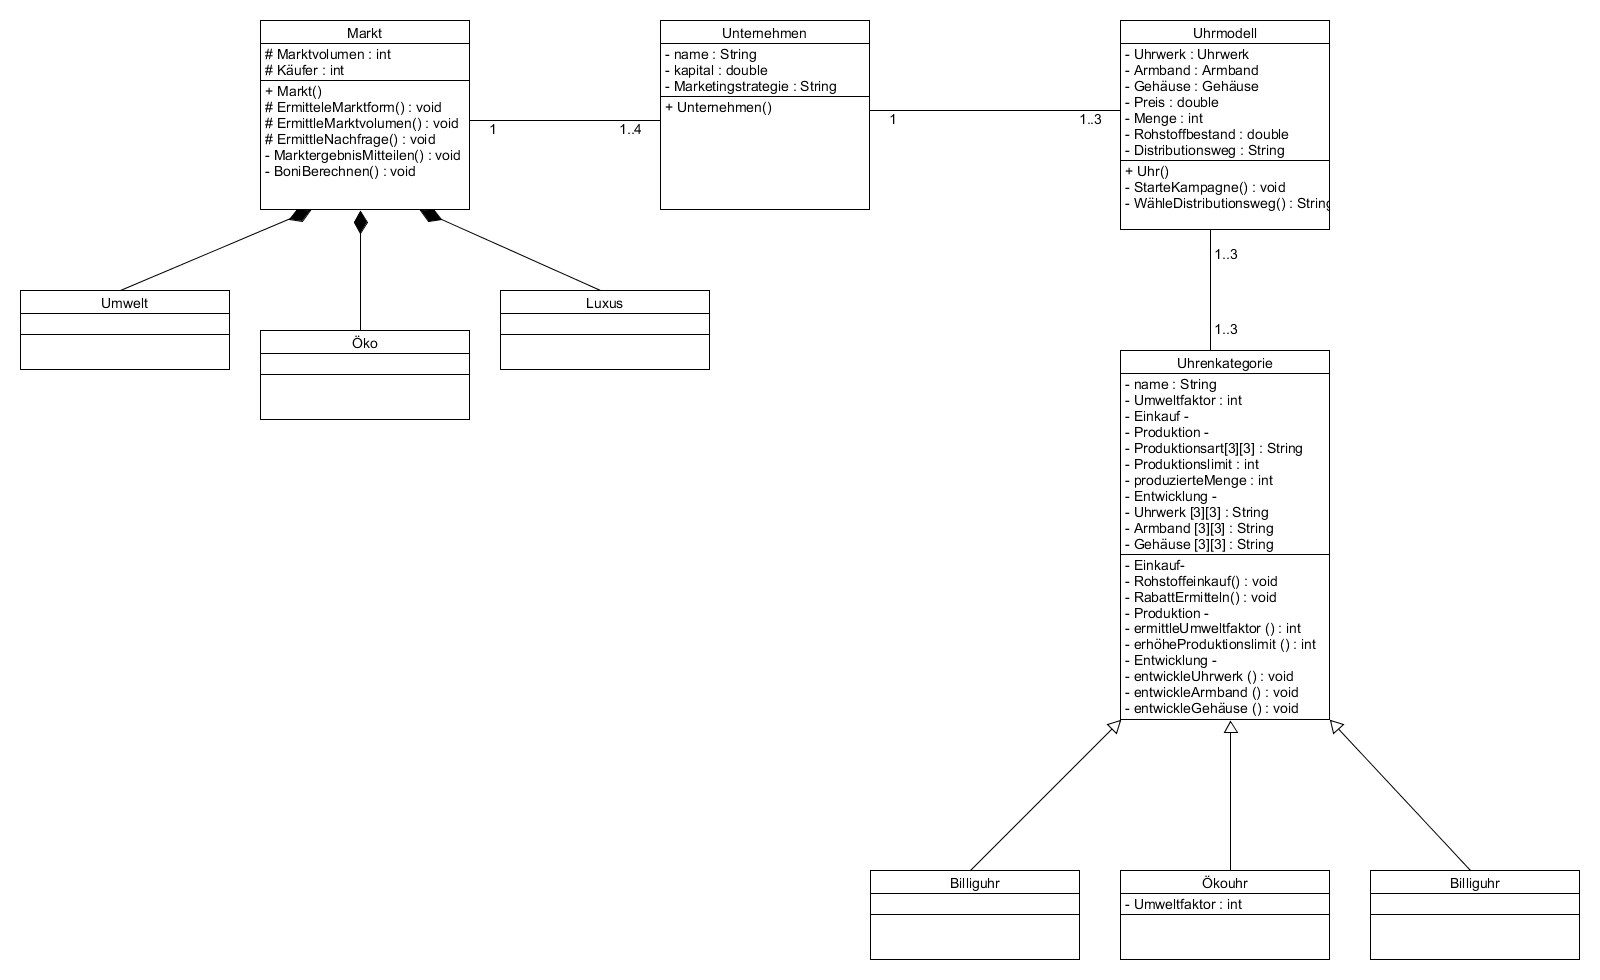
\includegraphics[scale=0.25, angle=90]{img/ErsterEntwurfUML.png} 
\end{figure}
\clearpage
\subsection{Finales UML/Unternehmenssimulation}
\begin{figure} [!h]
	\centering
	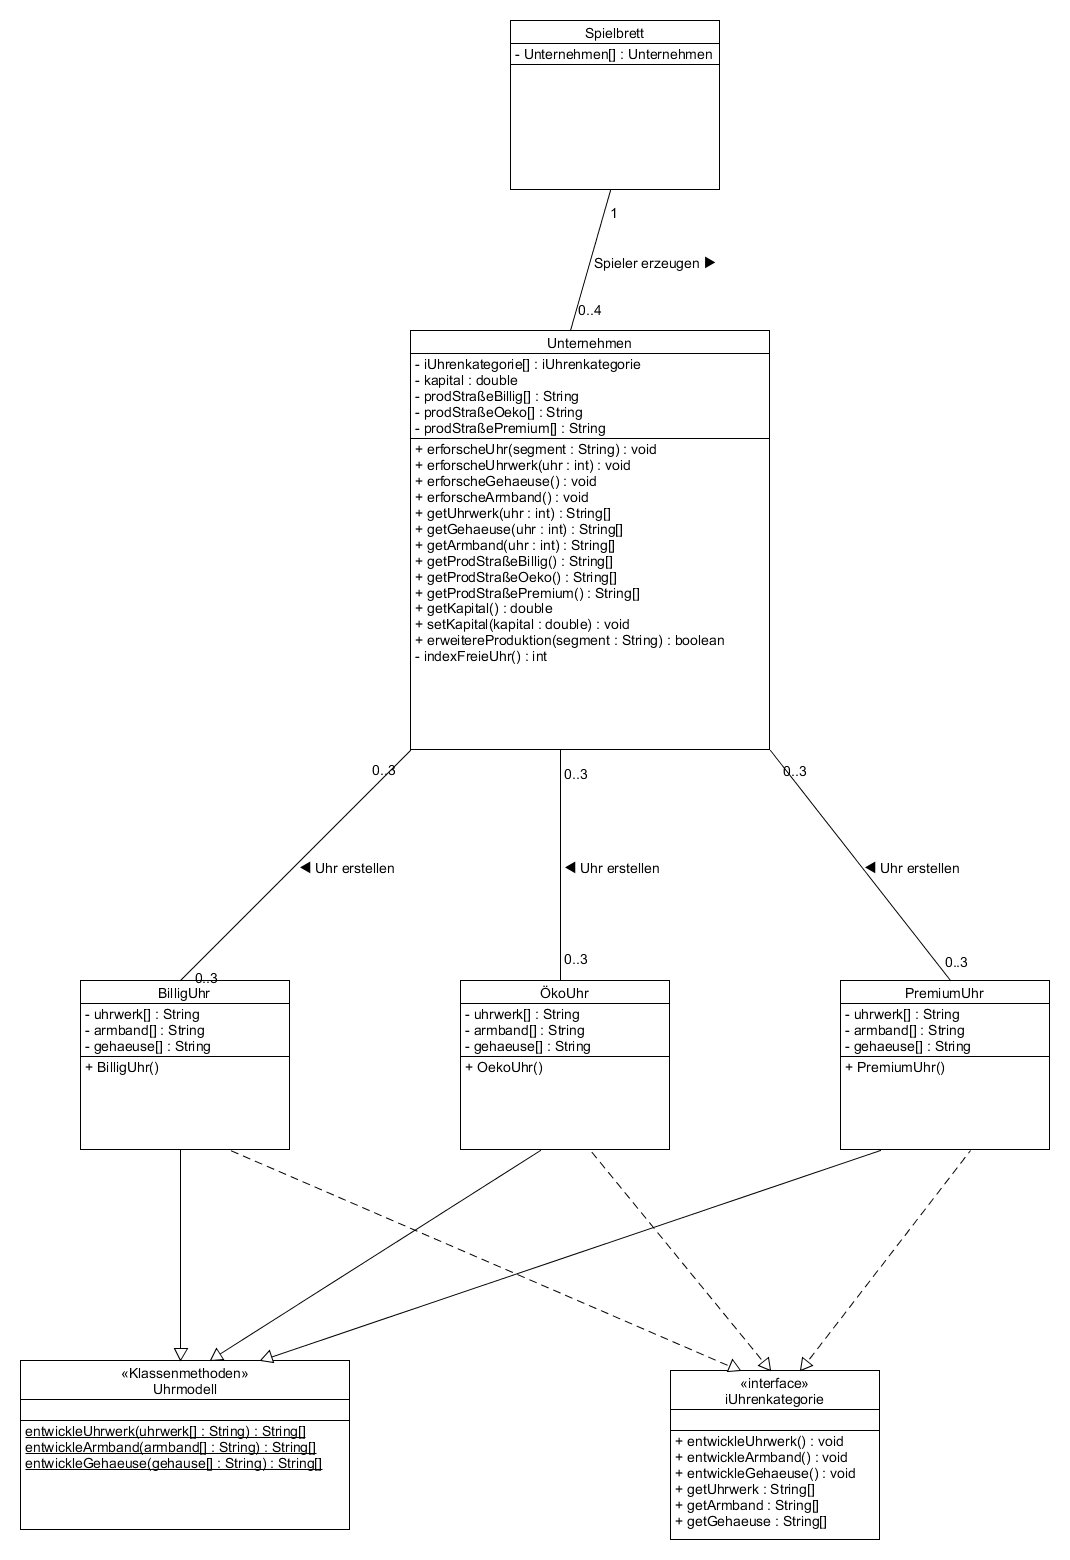
\includegraphics[scale=0.36]{img/Unternehmenssimmulation.png} 
\end{figure}
\clearpage
\section{Ablauf-UML}
\subsection{Spielablauf}
\begin{figure} [!h]
	\centering
	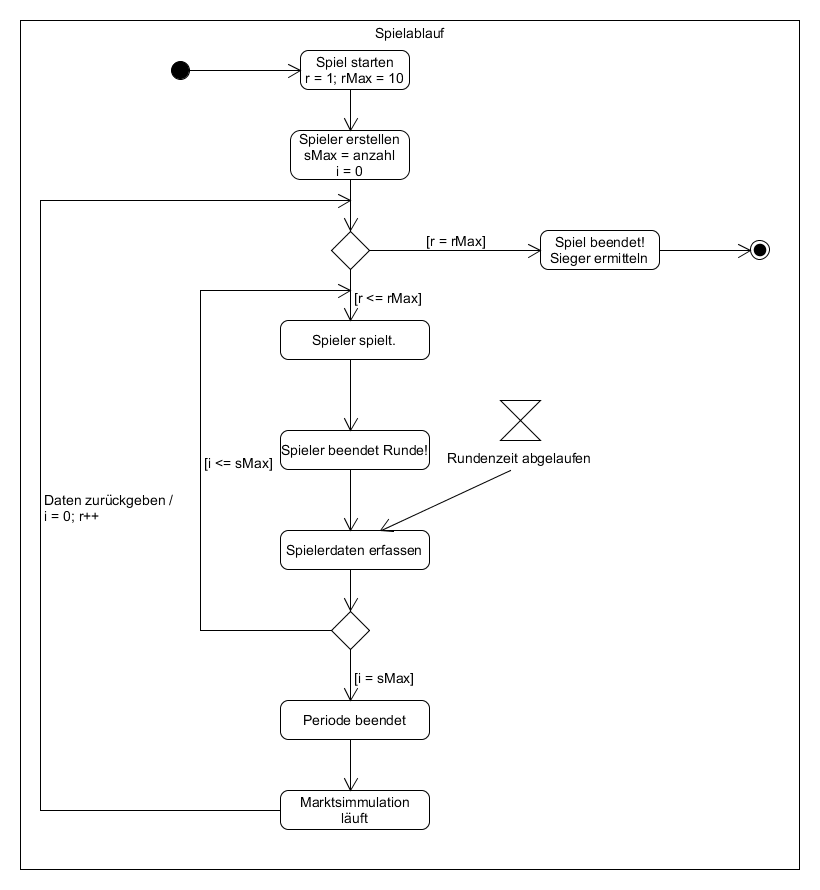
\includegraphics[scale=0.5]{img/Spielablauf.png} 
\end{figure}
\clearpage
\section{Markt-UML}
\subsection{Aufbau/Klasse Markt}
\begin{figure} [!h]
	\centering
	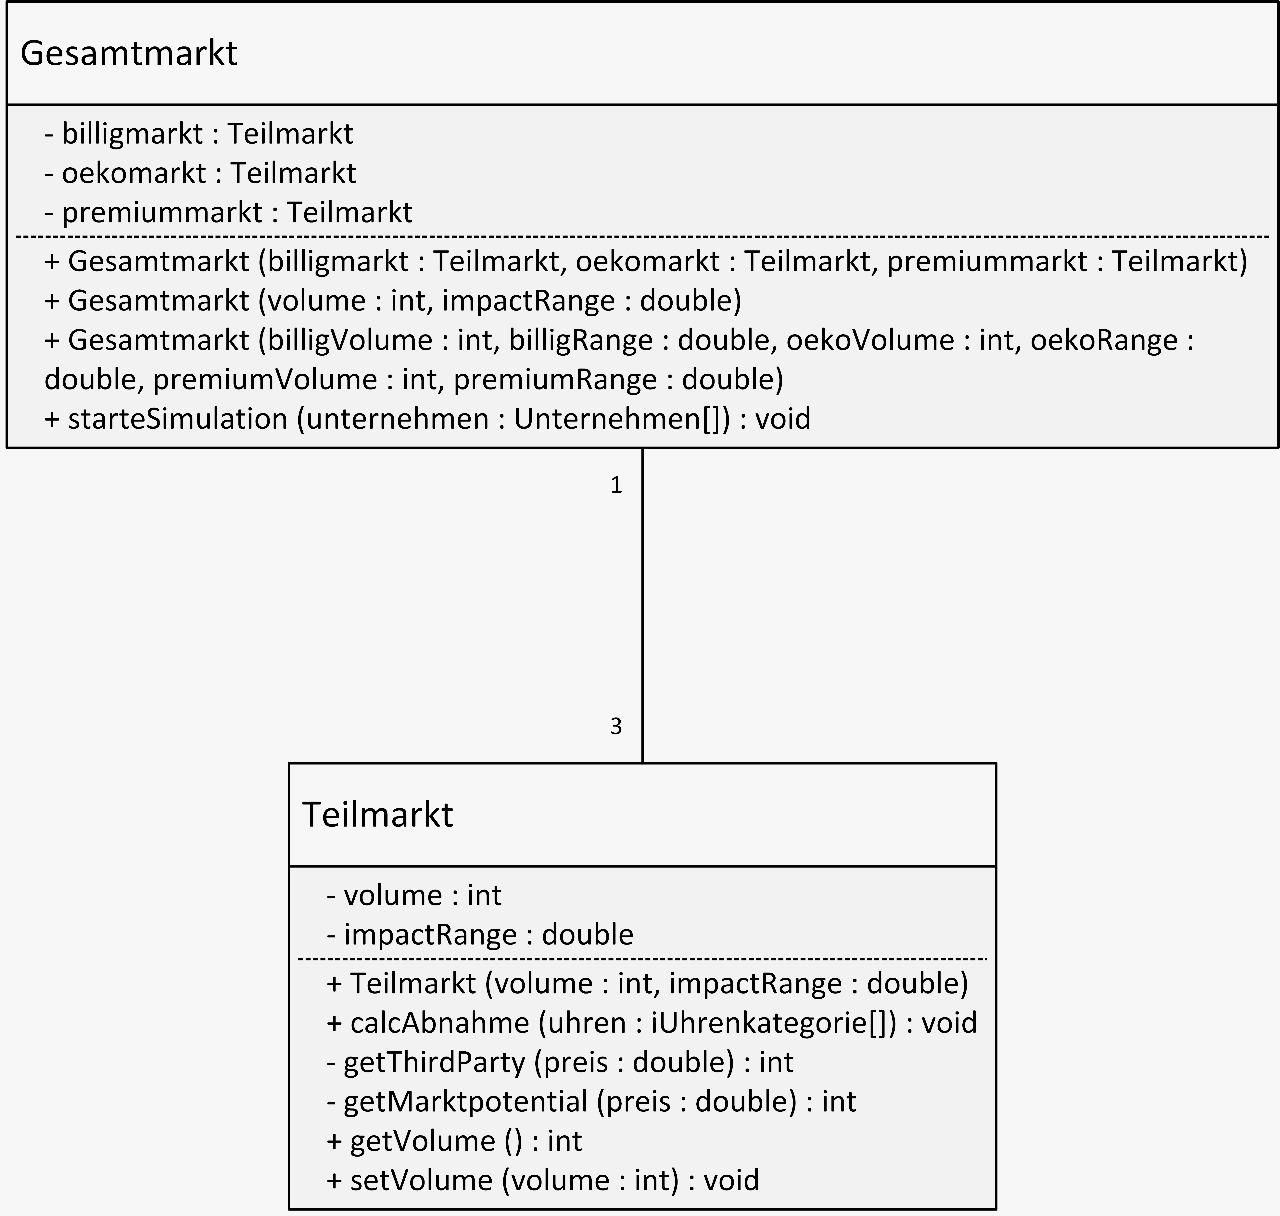
\includegraphics[scale=0.3]{img/Markt.png} 
\end{figure}
\clearpage
\begin{enumerate}
	\item ErmittleMarktform() 
	\begin{itemize}
	\item	
	\end{itemize}
	\item ErmittleMarktvolume() 
	\begin{itemize}
	\item 	
	\end{itemize}
	\item ErzeugeAngebotNachfrage() 
	\begin{itemize}
	\item 	
	\end{itemize}
	\item GetMarktergebnis() 
	\begin{itemize}
	\item 	
	\end{itemize}
	\item ErzeugeMarktkrise () 
	\begin{itemize}
	\item 	
	\end{itemize}
\end{enumerate}




